\documentclass{article}
\usepackage[utf8]{inputenc}
\usepackage{polski}
\usepackage{amsmath,amssymb,graphicx,subfig,pdfpages,enumitem,empheq,verbatim,csvsimple}
\usepackage{multirow}

\author{Krystian Baran 145000}
\title{Zadania z wykładu 10}

\begin{document}

\maketitle
\newpage

\tableofcontents
\newpage

% Zadanie 9
\section{Zadanie 9}
Dane z próby zostały pogrupowane w tabeli:
\begin{center} \begin{tabular}{|c|c|c|c|c|c|c|c|c|c|c|} \hline
Przedział & (0, 1] & (1, 2] & (2, 3] & (3, 4] & (4, 5] & (5, 6] & (6, 7] & (7, 8] & (8, 9] & (9, 10] \\ \hline
liczba i) &
52 & 38 & 20 & 12 & 7 & 6 & 5 & 5 & 4 & 1 \\ \cline{2-11}
wyników ii) & 33 & 36 & 19 & 14 & 9 & 8 & 4 & 6 & 5 & 4 \\ \hline
\end{tabular} \end{center}
Na poziomie istotności 0,02 zweryfikować hipotezę, że dane te
pochodzą z rozkładu o gęstości $f(x)$ określonej wzorem (wyznaczyć \textit{a}):
\[ f(x) = \left\{ \begin{array}{ccc} 
a(10 - x) & \text{dla} & x \in [0,10] \\
0 & \text{dla} & \text{w p. p.} 
\end{array} \right. \]

Wyznaczymy \textit{a} z własności funkcji gęstości:
\begin{align*}
\int_\mathbb{R} f(x) dx & = 1 \\
& = \int_\mathbb{R} a(10-x) \mathbb{I}_{[0,10]}(x) dx \\
& = \int_0^{10} a(10 - x) dx = a(10x - \frac{x^2}{2}) \Big\vert_0^{10} \\
& = a(100 - 50) = 50a = 1 \\
a & = \frac{1}{50} = 0.02
\end{align*}

Znając $a$ możemy wyznaczyć dystrybuantę:
\begin{align*} F(x) & = \int_{-\infty}^x 0.02(10 - t) \mathbb{I}_{[0,10]}(t) dt \\
& = \int_0^x 0.02(10 - t) dt \\
& = 0.02(10t - \frac{t^2}{2}) \Big\vert_0^x \\
& = 0.02(10x - \frac{x^2}{2})
\end{align*}

\[ F(x) = \left\{ \begin{array}{ccc}
0 & , & x < 0 \\
0.02(10x - \frac{x^2}{2}) & , & x \in [0,10] \\
1 & , & x > 10
\end{array} \right. \]

Wyznaczymy dystrybuantę z próby korzystając ze wzoru poniżej i biorąc lewe końce każdego przedziału:
\[ F_n(x|X) = \frac{1}{n} \sum_{k=1}^n \mathbb{I}_{(-\infty,x]}(X_k), x = 1,2,\dots, 10 \]

Poniżej przykładowe jedno obliczenie, wystarczy wziąć liczebność danego przedziału i poprzednich i podzielić przez całkowitą liczebność.
\[ F(1|X) = \frac{52}{150} \approx 0.346667 \]
\[ F(2|X) = \frac{52 + 38}{150} = \frac{90}{150} = 0.6 \] 
\[ \dots \]

Tak wyznaczono dystrybuantę dla $i$ i $ii$. Wartości zapisano poniżej wraz z wartosciami dystrybuanty wyznaczonej na początku
\begin{center} \begin{tabular}{|c|c|c|c|} \hline
$x$ & i) & ii) & F(x) \\ \hline
1 & 0.346667 & 0.239130 & 0.19\\ \hline
2 & 0.600000 & 0.500000 & 0.36\\ \hline
3 & 0.733333 & 0.637681 & 0.51\\ \hline
4 & 0.813333 & 0.739130 & 0.64\\ \hline
5 & 0.860000 & 0.804348 & 0.75\\ \hline
6 & 0.900000 & 0.862319 & 0.84\\ \hline
7 & 0.933333 & 0.891304 & 0.91\\ \hline
8 & 0.966667 & 0.934783 & 0.96\\ \hline
9 & 0.993333 & 0.971014 & 0.99\\ \hline
10 & 1.000000 & 1.000000 & 1\\ \hline
\end{tabular} \end{center}

\begin{center} \begin{tabular}{|c|c|} \hline
 & SUM n \\ \hline
i) & 150 \\ \hline
ii) & 138 \\ \hline
\end{tabular} \end{center}

Zastosujemy test Kołmogorowa, zatem musimy wyznaczyć wartość $D_n = max\{ |F_n(x|X) - F(x) | \}$, zatem obliczone zostały szukane różnice i wyznaczono wartości maksymalne wynoszące:
\begin{enumerate}[label = \roman*)]
\item 0.24
\item 0.14
\end{enumerate}

Korzystając z tablic wyznaczono wartości krytyczne:
\begin{align*}
\text{i) : } & \frac{1.51743}{\sqrt{150}} \approx 0.123898 \\
\text{ii) : } & \frac{1.51743}{\sqrt{138}} \approx 0.129172
\end{align*}

Widzimy zatem że wartości te są większe od wartości krytycznych, zatem odrzucamy hipotezę zerową mówiąca że wartości z próby mają podana dystrybuantę

\newpage
% Zadanie 13
\section{Zadanie 13}
Wygenerować próby o liczebności 100 obserwacji według rozkładów:
\begin{enumerate}[label = \roman*)]
\item $N(900;50)$,
\item $TR(725;1075)$,
\end{enumerate}
Następnie
\begin{enumerate}[label = \alph*)]
\item obliczyć podstawowe statystyki,
\item sporządzić wykresy histfit, normplot, Q-Q,
\item przeprowadzić testy losowości,
\item przeprowadzić testy normalności,
\item przeprowadzić testy zgodności z innymi rozkładami,
\item przeprowadzić test zgodności dla wygenerowanych prób.
\end{enumerate}

Dane losowe wygenerowane w R za pomocą funkcji poniżej. Zaokrąglono wartości do dwóch liczb po przecinku.
\begin{itemize}
\item \textbf{rnorm(100, 900, 50)}
\item \textbf{rtri(725, 1075, (1075-725)/2 + 725)} (pakiet "EnvStats")
\end{itemize}
Wartości prób losowych podane pod zakładką \textbf{Dane}.

\subsection{a)}
Korzystając z gotowych funkcji w R, obliczono średnią, wariancje i odchylenie standardowe. Wyniki zapisano poniżej.
\begin{itemize}
\item \textbf{mean()} - średnia
\item \textbf{var()} - wariancja
\item \textbf{sqrt(var())} - odchylenie standardowe
\end{itemize}

\begin{center} \begin{tabular}{|c|c|c|} \hline
 & i) & ii) \\ \hline
$\overline{X}$ & 896.18 & 899.5525 \\ \hline
$S^2$ & 2485.676 & 4611.553 \\ \hline
\end{tabular} \end{center}

\subsection{b)}
Nie rysowano.

\subsection{c)}
Aby zbadać losowość próby zastosujemy test Walda Wolfowitza. Wyznaczymy statystykę następująco:
\[ Z = \frac{R - \mu_R}{\sigma_R} \]
Statystyka ta ma rozkład statystyki $\sim N(0,1)$. $R$ jest liczbą serii która wyznaczamy jako ilość liczb mniejszych od mediany.
\begin{align*}
\mu_R &= \frac{2 \cdot n_1 \cdot n_2}{n_1 + n_2} + 1 \\
& = \frac{2 \cdot 50 \cdot 50}{50 + 50} + 1 \approx 51 \end{align*}

\begin{align*}
\sigma^2_R & = \frac{2 \cdot n_1 \cdot n_2 \cdot (2 \cdot n_1 \cdot n_2 - n_1 - n_2)}{(n_1+n_2)^2(n_1 + n_2 - 1)} \\
& = \frac{2 \cdot 50 \cdot 50 (2 \cdot 50 \cdot 50 - 50 = 50)}{(50 + 50)^2(50 + 50 - 1)} \approx 24.747475 \end{align*}

\[ \sigma_R = \sqrt{\sigma^2_R} \approx 4.974683 \]

Wtedy, ponieważ R jest równe dla oby danych i wynosi 50:
\[ Z = \frac{50 - 51}{4.974683} \approx 0.201018 \]

Obliczymy \textit{p-value} dla prawostronnej i lewostronnej hipotezy o losowości:
\[ \text{p-value}_1 \overset{R}{=} pnorm(0.201018, 0, 1) \approx 0.5796578 \]
\[ \text{p-value}_2 \overset{R}{=} 1 - pnorm(0.201018, 0, 1) \approx 0.4203422 \]

W oby przypadkach nie możemy odrzucić hipotezę że wartości pochodzą z próby losowej.

\subsection{d)}
Test normalności został przeprowadzony za pomocą funkcji w R \textbf{ks.test(x,test)}, gdzie \textbf{test} jest dystrybuantą:
\begin{itemize}
\item $F_{N(900,50)}$ dla i)
\item $F_{N(\overline{X},s)}$ dla ii)
\end{itemize}

Test jest dwustronny i oddaje wartości \textit{p-value}, odpowiednio, 0.7774 dla \textbf{i)}, 0.8638 dla \textbf{ii)}. Zatem, przyjmując $\alpha = 0.05$ nie możemy odrzucić hipotezę o normalności. Wnioskujemy że oba rozkłady są normalne. \\
Ponieważ drugi rozkład pochodzi od rozkładu trójkątnego, możemy powiedzieć że tego typu rozkład jest zbliżony do normalnego.

\subsection{e)}
Nie przeprowadzono testu.

\subsection{f)}
Jak w podpunkcie \textbf{d}, zastosujemy test Kołmogorowa w R następująco: \textbf{ks.test{x,y}}. Gdzie $x$ są dane pierwszej próby a $y$ są dane drugiej próby. Orzymano następujący wynik: \\
\textbf{
Two-sample Kolmogorov-Smirnov test \\
data:  x and y \\
D = 0.13, p-value = 0.3667 \\
alternative hypothesis: two-sided \\
}

\textit{p-value} jest większe od $\alpha$, zatem wnioskujemy że rozkłady są do siebie podobne. Natomiast, z tabeli w \textbf{Tabele} weźmiemy wartość $D_n$ dla n = 100, uzyskamy:
\[ D_n = \frac{1.35810}{\sqrt{100}} = 0.13581 \]
Zatem widzimy że rozkłady są bardzo blisko bycia rożnych, ponieważ  gdy $D_n < D$ to odrzucamy hipotezę równania się rozkładów.



\newpage
% Zadanie 18
\section{Zadanie 18}
Wygenerować dużą próbę według jednego z rozkładów: beta, gamma, Weibulla lub logarytmiczno-normalnego i przekazać uzyskane dane drugiej osobie do identyfikacji rozkładu – nie informując o mechanizmie generowania. Dokonać oceny jakości dokonanej identyfikacji. \\ \par

Uzyskane dane załadowano w R i, za pomocą funkcji w pakiecie "moments" obliczono współczynnik asymetrii.
\[ \tilde{\mu}_3 = \frac{\mu_3}{\sigma^3} \overset{R}{=} skewness(data) \approx 3.454167 \]
Jest to wartość dodatnia, zatem rozkład danych może być logarytmiczno-normalny, Weibulla lub gamma.

Aby przeprowadzić testy skorzystano z następującego skryptu w R, który oblicza dystrybuantę dla podanych danych, dokonuje "fitdistr" dla danego rozkładu testowego, oblicza wartość $D_{n,\alpha}$ na poziomie $\alpha = 0.05$ według tablicy w \textbf{Tablice} i oblicza $D_n = max\{|F_n(x) - F(x)|\}$.
{\fontfamily{pcr}\selectfont
\begin{tabbing}
library("moments") \\
library("MASS") \\
data = read.csv("data.csv") \\
x = sort(data[[1]]) \\
D = 1.3581/sqrt(length(x)) \\
cat("Skewness = ", skewness(x), "$\backslash$ n") \\
\# Dystrybuanta empiryczna \\
X = c() \\
s = 0 \\
for\=(i in x) \{ \+
	s = length(which($x <= i$))/length(x) \\
	X = c(X, s) \- \\
\} \\
\\
\# Weibull \\
estimate = fitdistr(x,"weibull") \\
k = estimate[[1]][1] \\
lambda = estimate[[1]][2] \\
Y = pweibull(x, k, lambda) \\
d0 = max(abs(X-Y)) \\
cat("D0 = ", d0, " D = ", D, "$\backslash$n") \\
\\
\# gamma \\
estimate = fitdistr(x,"gamma") \\
alpha = estimate[[1]][1] \\
sigma = estimate[[1]][2] \\
Y = pgamma(x, alpha, rate = sigma) \\
d0 = max(abs(X-Y)) \\
cat("D0 = ", d0, " D = ", D, "$\backslash$ n") \\
\\
\#lognormal \\
estimate = fitdistr(x,"lognormal") \\
meanlog = estimate[[1]][1] \\
sdlog = estimate[[1]][2] \\
Y = plnorm(x, meanlog, sdlog) \\
d0 = max(abs(X-Y)) \\
cat("D0 = ", d0, " D = ", D, "$\backslash$n")
\end{tabbing}}

Wynik tego skryptu jest następujący: 
\begin{itemize}
\item Skewness =  3.454167 
\item (Weibull) D0 =  0.06315938  D =  0.03036804 
\item (gamma) D0 =  0.07382558  D =  0.03036804 
\item (lognormal) D0 =  0.008872974  D =  0.03036804 
\end{itemize}
Aby wiedzieć czy dane mają podaną rozkład porównujemy $D$ z $D0$, jeżeli $D$ jest większe od $D0$ to przyjmujemy że dane mają podany rozkład, w przeciwnym wypadku nie mają danego rozkładu. Widzimy zatem że dla Rozkładu Weibulla i gamma $D < D0$ zatem dane nie mają żadne z tych danych; natomiast widzimy że dla rozkładu logarytmiczno normalnego $D > D0$, zatem wnioskujemy że dane mają rozkład logarytmiczno normalny.


\newpage
% Tablice
\section{Tablice}
 
Tablica wartości $D_{n,\alpha}$ testu Kołmogorowa.
\begin{figure}[h!] \begin{center}
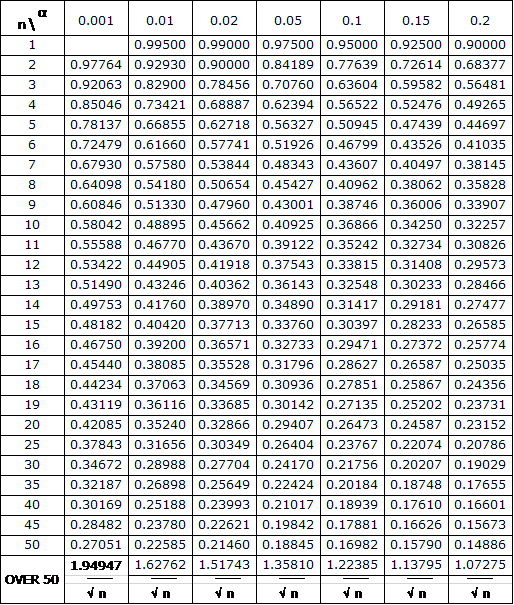
\includegraphics[height=0.5\textheight, angle=0]{"pdf/tablicaK.png"}
\end{center} \end{figure}

\newpage
\section{Dane}

\begin{center}
\tiny
\csvreader[tabular = |c|c|,
table head = \hline \bfseries{Lp} & \bfseries{x} \\ \hline,
late after last line = \\ \hline]{w10zad13LaTex.csv}{}{\csvlinetotablerow}
\end{center}

\newpage
\begin{center}
\tiny
\csvreader[tabular = |c|c|,
table head = \hline \bfseries{Lp} & \bfseries{x} \\ \hline,
late after last line = \\ \hline]{w10zad13_TRLaTex.csv}{}{\csvlinetotablerow}
\end{center}

\newpage
% Bibliografia
\section{Bibliografia}
\begin{itemize}
\item https://en.wikipedia.org/wiki/Kolmogorov\%E2\%80\%93Smirnov\_test
\item https://www.real-statistics.com/statistics-tables/kolmogorov-smirnov-table/
\item https://www.real-statistics.com/tests-normality-and-symmetry/statistical-tests-normality-symmetry/kolmogorov-smirnov-test/
\item https://kindsonthegenius.com/blog/how-to-perform-wald-wolfowitz-test-testing-for-homogeneity-with-run-test/
\end{itemize}

\end{document}